\documentclass[twoside]{memoir}
\usepackage{nus-el-ht}
% Hyperref enables click-through hyperlinks in your PDF. The hyphens option indicates where to break long URLs. 
\PassOptionsToPackage{hyphens}{url}\usepackage{hyperref}
%\usepackage{hyperref}
% The Latin Modern font is a modernised replacement for the classic Computer Modern. Feel free to replace this with a different font package.
\usepackage{lmodern}

% We use setspace to implement double-spacing, but with a specific command to leave quotes single-spaced. 
\DisemulatePackage{setspace}\usepackage{setspace}
\expandafter\def\expandafter\quote\expandafter{\quote\singlespacing}
\doublespacing

% Linguistics-specific packages.
% For typing IPA.
\usepackage{tipa} 
\newcommand{\phonem}[1]{\textipa{/#1/}}
\newcommand{\phonet}[1]{\textipa{[#1]}}
% For drawing syntax trees.
\usepackage{qtree}\usepackage{tikz} 
\usepackage{tikz-qtree}
\tikzset{every tree node/.style={align=center,anchor=north}}
% For typesetting and labelling examples, incl. glossed examples. 
\usepackage{expex} 
\lingset{Everyex=\singlespace}

\setlength\parindent{0pt}

% Titling commands. 
\title{Honours Thesis Template}
\author{Ng Wei Le}
\supervisor {Assistant Professor Subhroshekhar Ghosh}
\degree{Bachelor of Science with Honours}
\faculty{Faculty of Science}
\dept{Mathematics}
\date{\today}

\begin{document}
	% First, we go into "front matter" mode.
	% Among other things, this gives us Roman page numbers.
	\frontmatter
	
	% We tell LaTeX to make a title page, sections for acknowledgements, the abstract, and the table of contents (important!). 
	
\maketitle

\chapter{Acknowledgement}
Special thanks to my research supervisor, Prof. Subhroshekhar Ghosh, for guiding me in the direction to take the research, and for the time he spent teaching me the concepts.
	
\begin{abstract}
	The bias-variance tradeoff is a tenet of classical Machine Learning practice, where the algorithm tries to balance the error from the bias term and variance term, typically by means of controlling the richness of the model to find a sweet spot between underfitting and overfitting. However, in many modern Machine Learning practices, the model is made to highly overfit the data, even up till the point of near interpolation. This is done even under the conditions of large amounts of data and noise.\\
	The papers discussed in this thesis show that this happens not only in deep learning, but also kernel machines with close to 0 training error, and why current generalization bounds do not explain such phenomenon well. Additionally, a paper proposes a possible performance curve to explain how overfitting could be beneficial, and some empirical evidence to support this.
\end{abstract}
	
\tableofcontents

% Include the list of figures and list of tables only if you actually have figures and tables! (The * after each indicates that it should not be included in the table of contents.)
\listoffigures*
%\listoftables*

% Next, we go into "main matter" mode.
% This resets the page numbers and uses Arabic numerals.
\mainmatter

\chapter{Introduction}

\section{Supervised Learning}
Given a set of (training) datapoints $\{(x_1,y_1), ..., (x_n,y_n)\}$ where $x_i \in \RR^d$ and $y_i \in \RR$ for $1 \leq i \leq n$, and assuming $(x_i, y_i)$ were independent and identically distributed variables drawn from a probability distribution $Q$, we want to find a predictor function $h_n:\RR^d \rightarrow \RR$ that predicts $y$ "well" given $x$ that has not been seen.\\
To represent how well this function predicts, let $l$ represent a loss function. Examples include the squared-loss function $l(y,\hat{y}) = (\hat{y} - y)^2$, and the 0-1 loss, usually used for classification: $l(\hat{y},y) = 1_{\hat{y} \neq y}$.\\
The general goal of (supervised) machine learning to find a function $h$ that minimizes the expected loss: $\EE_{x,y}[l(h(x), y)]$.\\
In Empirical Risk Minimization (ERM), given datapoints $\{(x_1,y_1), ..., (x_n,y_n)\}$, the goal is to find a function $h_n$ in some class of function $\HH$  to minimize the empirical risk: 
\[L_{emp}(h_n) = \frac{1}{n} \sum_{i=1}^{n} l(h_n(x_i), y_i). \]
Intuitively, if a function $h_n$ does not predict training data well (has a high $L_{emp}(h_n)$), this would tell us that it will not predict other $(x,y)$ samples drawn randomly as well. 

The empirical risk minimizer, $\hat{h}: \RR^d \rightarrow \RR$ is then defined by:
\[ \hat{h_n} = \arg\min_{h_n \in \HH} L_{emp}(h_n). \]
Classically, there are reasons why one does not tend to choose a function $h_n$ that reduces the empirical loss to near zero values, typically due to bounds on the generalization gap.

\section{Bias Variance Tradeoff}
We define the generalization error (or sometimes known as the generalization gap) as difference between the empirical and expected classifier loss, i.e. $ \abs{ \EE_{x,y}[l(\hat{h_n}(x), y)] - L_{emp}(\hat{h_n}) } $. It would make sense to decrease this gap to as little as possible.\\
Many classical bounds have this generalization gap is a form of:
\begin{equation} \label{eqn:Generalization_Gap}
\EE_{x,y}[l(\hat{h_n}(x), y)] \leq L_{emp}(\hat{h_n}) + O(\sqrt{c/n})
\end{equation}
where $c$ is some  measure of the complexity of $\HH$, for example the fat-shattering dimension, VC-dimension, Rademacher complexity, etc. The general result being that, with a greater complexity of the function class $\HH$, the greater the upper bound of this generalization gap. However, if $\HH$ is not complex enough, we may not find any function $\hat{h_n} \in \HH$ that reduces the empirical risk sufficiently (underfitting). Hence, classical algorithms try to find a balance between over and underfitting, decreasing the expected loss by controlling $\HH$, either explicitly or implicitly.
For example, to change the complexity of $\HH$ explicitly, one might choose a simpler or more complicated architecture for a neural network. To reduce the complexity of $\HH$ implicitly, one might user regularization to  penalize coefficients to limit the model complexity, or simply stop the training algorithm prematurely (early stopping).

This classical curve from \cite{Belkin_2019} is shown in Figure \ref{fig:Classical_Descent}.
\begin{figure}
	\centering
	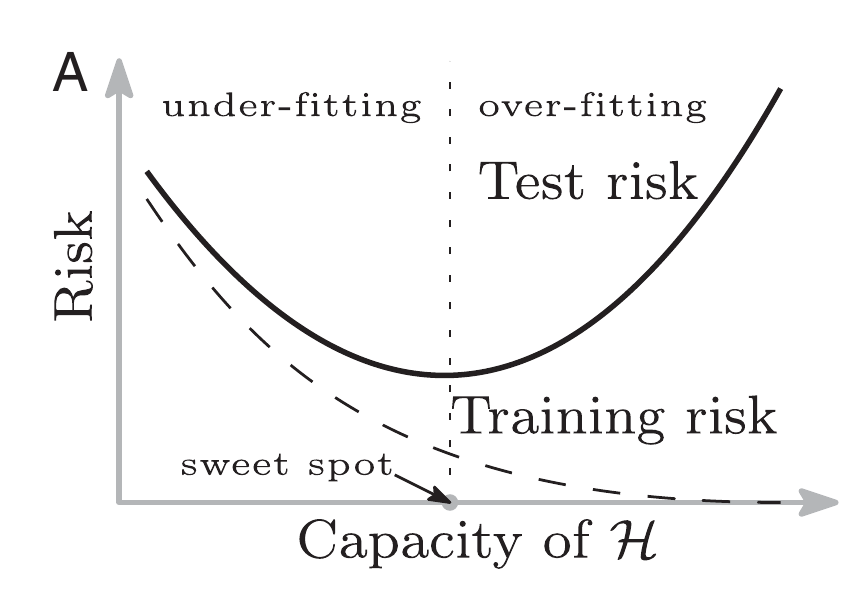
\includegraphics[width=1.2\textwidth]{"Images/Classical_Descent.png}
	\par
	\caption{Curve showing how the training and test risk changes with respect to the capacity of $\HH$. The test risk results from bias-variance tradeoff, and the Capacity of $\HH$ is selected at the sweet spot.} \label{fig:Classical_Descent}
\end{figure}

\section{Modern Machine Learning}
In a paper by \cite{Zhang_Deep_Learning}, examples were given where  deep neural networks were trained to the point of little to no training error. Different architectures were tested on the CIFAR10 dataset (\cite{krizhevsky2009learning}) and ImageNet dataset (\cite{Russakovsky_2015}). However, very accurate predictions on the new data was given.\\
In \cite{Alfredo2016}, the architectures used on ImageNet have large amounts of parameters, multiple times bigger than the number of training datapoints.

\section{Research Question}

Indeed, it is still unanswered as to why these overparameterized data do not seem to cause high test loss due to overfitting. The papers discussed further show empirically that this property is not exclusive to deep learning, but also seems to appear in learning for kernel machines as well. This will be followed by a plausible explanation on how the classical bias-variance tradeoff graph can be reconciled with modern methods.\\
We first give a brief introduction on kernels and Reproducing Kernel Hilbert Spaces.

\chapter{Kernels}
	\section{Notation}
	We use the symbol $\KK$  when it can refer to both $\RR$ or $\CC$. Also, let $z^*$ or $(z)^*$ denote the conjugate of $z$ for any $z \in \CC$.
	The sections covering Kernels and reproducing kernel Hilbert spaces are heavily referenced using Steinwart, Christman \cite{steinwartSVM}.
	
	\section{Definition and Properties}
	\begin{defn}
		For a non-empty set $X$, let $k: X \times X \rightarrow \KK$ be known as a kernel if there exists a function $\phi: X \rightarrow \mathcal{H}$ (known as a feature map of k) where $\mathcal{H}$ is a $\KK$-Hilbert space (known as a feature space of k) such that
		\begin{equation}
		k(x_1, x_2) = \inner{\phi(x_2), \phi(x_1)}_\mathcal{H}.
		\end{equation}
	\end{defn}
	
	\begin{lem} \label{lem:kernelSymm}
		For any kernel $k$ on $X$, $k(x_1, x_2) = k(x_2, x_1)^*$.
	\end{lem}
	
	From the properties of the inner product, we know that $k(x_1, x_2) = \inner{\phi(x_1), \phi(x_2)}^* = k(x_2, x_1)^*$. Therefore, for kernels on $\RR$, the symmetric property: $k(x_1, x_2) = k(x_2, x_1)$ holds.
	\begin{lem}
		Let $k_1, k_2$ be kernels on a non-empty set $X$. Then $k_1 + k_2$ and $ak_1, a \in \RR^+ \cup \{0\}$ are kernels. 
	\end{lem}
	Below, we define the Gaussian RBF kernel:
	\begin{defn}
		Let the complex Gaussian RBF kernel (on $\CC^d$)be defined as:
		\[ k_{\gamma, \CC^d}(z, z') := e^{-\gamma^{-2} \sum_{i=1}^{d} (z_i - z_i'^*)^2 } .\]
		We then define the real Gaussian RBF kernel (or simply the Gaussian RBF kernel for short) acting on $\RR^d$ as:
		\[ k_\gamma(x, x') = e^{- \gamma^{-2} \norm{x - x'}_2^2} \]
	\end{defn}
	It can be shown (\cite{steinwartSVM}) that the complex and real Gaussian RBF kernels are kernels.
	\begin{defn}
		For a non-empty set $X$, a function $k: X \times X \rightarrow \RR$ is said to be a positive definite if, for any $m \in \ZZ^+ \cup \{0\}$ and all $x_1, ..., x_n \in X$, we have the following matrix (called the Gram matrix) being positive semi-definite:
		\[ K := (k(x_i, x_j))_{i,j}. \]
		Equivalently: for all $a_1, ..., a_n \in \RR$, we have:
		\[ \sum_{j=1}^{n} \sum_{i=1}^{n} a_j a_i k(x_j, x_i). \]
	\end{defn}
	\begin{defn}
		The positive definite function $k: X \times X \rightarrow \RR$ is said to be symmetric if  $k(x_1, x_2) = k(x_2, x_1)$ for all $x_1, x_2 \in X$
	\end{defn}
	\begin{thm}
		A real function $k:X \times X \rightarrow \RR$ is a kernel if and only if $k$ is a positive definite symmetric function (also known as a positive definite kernel).
	\end{thm}
	\begin{proof}
		Suppose k is a kernel. Then there exists some feature map $\Phi: X \rightarrow \HH$.
		\begin{equation*}
		\begin{split}
		\sum_{j=1}^{n} \sum_{i=1}^{n} a_j a_i k(x_j, x_i) &= 
		\sum_{j=1}^{n} \sum_{i=1}^{n} a_j a_i \inner{\phi(x_i), \phi(x_j)}_\HH \\
		&= \inner{\sum_{i=1}^{n} a_i \phi(x_i), \sum_{j=1}^{n} a_j \phi(x_j)}_\HH \\
		&= \norm{\sum_{i=1}^{n} a_i \phi(x_i)} \\
		&\geq 0.
		\end{split}
		\end{equation*}
		Also, from Lemma \ref{lem:kernelSymm}, we know that the real kernel $k$ is symmetric, proving one side of the theorem. To prove the other side: \\
		Given $k:X \times X \rightarrow \RR$ a positive definite symmetric function, we prove that $\Phi: X \rightarrow H$ where $x \mapsto k(\cdot, x)$ is a valid feature map for some feature space $H$. First, we define
		\[ \hat{\HH} := \sum_{i=1}^{n} a_i k(\cdot, x_i), n \in \nonNegInt, a_i \in \RR \text{ for all } i, x_i \in X \text{ for all } i. \]
		For $f, g \in \hat{\HH}$ where $f = \sum_{i=1}^{n}a_i k(\cdot, x_i)$ and $g = \sum_{j=1}^{m}b_j k(\cdot, y_j)$, we define the inner product as such:\
		\begin{equation} \label{eqn:innerKernel}
		\begin{split}
		\inner{f, g}  &:= \sum_{i=1}^{n} \sum_{j=1}^{m} a_i b_j k(y_j, x_i) \\
		&= \sum_{j=1}^{m} b_j f(y_j) \\
		&= \sum_{i=1}^{n} a_ig(x_i) 
		\end{split}
		\end{equation}
		This definition is bilinear and symmetric. \\
		We also have: $\inner{f, f} = \sum_{i=1}^{n}\sum_{j=1}^{n}a_i a_j k(x_j, x_i) \geq 0 $ since k is a positive definite function. It can be shown that $\inner{\cdot, \cdot}$ follows Cauhy-Schwarz Inequality (\cite{steinwartSVM}), hence we have:
		\begin{equation*}
		\begin{split}
		|f(x)|^2 &= |\sum_{i=1}^{n}a_ik(\cdot, x_i)|^2 \\
		&= |\inner{f, k(\cdot, x)}|^2 ~ (\because (\ref{eqn:innerKernel}) \text{ with } g = \sum_{j=1}^{m}b_j k(\cdot, y_j) = k(\cdot, x) \text{ with } m=1, b_1 = 1, y_1 = x)\\
		&\leq \inner{k(\cdot, x), k(\cdot, x)} ~ \inner{f, f}. 
		\end{split}
		\end{equation*}
		Therefore, if $\inner{f, f} = 0$, then $f = 0$, hence showing that $\inner{f, f} > 0$ if and only if $f \neq 0$. Hence, $\inner{\cdot, \cdot}$ defines a proper inner product in $\hat{\HH}$. \\
		Let $\HH$ be the completion of $\hat{\HH}$ and the map $U: \hat{\HH} \rightarrow \HH$ be the map where $\inner{Ux, Uy}_{\HH} = \inner{x, y}_{\hat{\HH}} $ for all $x, y \in \hat{\HH}$. Then we have, for all $x, x' \in X$:
		\[ k(x, x') = \inner{k(\cdot, x'), k(\cdot, x)} _{\hat{\HH}} = \inner{Uk(\cdot, x'), Uk(\cdot, x)}_{\HH} \]. Thus we find a feature map of $k$, proving that $k$ is a kernel.
	\end{proof}
	
	\section{Reproducing Kernel Hilbert Spaces} \label{sec:RKHS}
	Initially introduced by Stanislaw Zaremba, reproducing kernel Hilbert spaces have many applications in the fields such as Statistical Learning and complex analysis. An RKHS is a $\KK$-Hilbert function space where point evaluation is continuous linear funcitonal.
	\begin{defn}
		\textbf{(RKHS).} Let $\mathcal{H}$ be a $\KK$-Hilbert space of functions over a non-empty set $X$. $\HH$ is called an RKHS over $X$ if the Dirac function $\delta_x: \HH \rightarrow \KK$ defined as:
		\[ \delta_x(f) := f(x), ~ x \in X, ~ f \in \HH \] is continuous.
		Equivalently, there exists $ 0 < M_x < \infty $ such that
		\[ \delta_x(f) \leq M_x \norm{f}_\mathcal{H}, ~ \text{for all} f \in \HH. \]
		$\delta_x$ is called a bounded operator on $\HH$.
	\end{defn}
	
	This is not easy to put into practice, hence the reproducing kernel is defined.
	\begin{defn} \textbf{(Reproducing Kernel).}
		For a non-empty set $X$ and a function $k : X \times X \rightarrow \KK$ where $k(\cdot, x) \in \HH$ for all $x \in X$ and the following property hold for all $x in X$ and $f \in \HH$:
		\begin{equation} \label{eqn:ReproducingProp}
		f(x) = \inner{f, k(\cdot, x)}
		\end{equation}
		The condition in equation (\ref{eqn:ReproducingProp}) is also known as the reproducing property.
	\end{defn}
	\begin{defn} \label{def:CanFeatureMaps}
		\textbf{(Canonical Feature Maps).}
		Let $\mathcal{H}$ be an RKHS over $X$ with reproducing kernel $k$. Let the function $\Phi: X \rightarrow \mathcal{H}$ be defined such that for all $x \in X$,
		\[ \Phi(x) = k(\cdot, x). \]
		We call $\Phi$ the canonical feature map of $k$.
	\end{defn}
	\begin{lem}
		\textbf{(A reproducing kernel of an RKHS is a kernel).}
		Let $\mathcal{H}$ be an RKHS over $X$ with reproducing kernel $k$. Then $k$ is a kernel.
	\end{lem}
	\begin{proof}
		We simply proof that $\Phi$ is a feature map of $k$.
		\begin{equation*}
		\begin{split}
		\inner{\Phi(x_2), \Phi(x_1)} &= \inner{k(\cdot, x_2), k(\cdot, x_1)} \\
		&=  k(x_1, x_2) ~ (\because \text{Reproducing Property } (\ref{eqn:ReproducingProp}))
		\end{split}
		\end{equation*}
		So $\mathcal{H} is also a feature space of k$.
	\end{proof}
	\begin{lem}
		Let $\mathcal{H}$ be an $\KK$-Hilbert functional RKHS over $X$ with reproducing kernel $k$. Then $H$ is a Reproducing Kernel Hilbert Space.
	\end{lem}
	\begin{proof}
		Recall the Dirac functional $\delta_x: H \rightarrow \KK$ where:
		\[ \delta_x(f) = f(x), ~ x \in X, ~ f \in H. \]
		Then we have:
		\begin{equation*}
		\begin{split}
		|\delta_x(f)| &= |f(x)| \\
		&= |\inner{f, k(\cdot, x)}| ~ (\because \text{Reproducing Property }(\ref{eqn:ReproducingProp})) \\
		&\leq \norm{k(\cdot, x)}_\mathcal{H} \norm{f}_
		\mathcal{H} ~ (\because \text{Cauchy-Schwarz Inequality}) \\
		\end{split}
		\end{equation*}
		This shows that the Dirac functionals are continuous.
	\end{proof}
	
	\subsection{Representer Theorem} \label{subsec:RepThm}
	Representer Theorem ensures that the $argmin$ of an empirical risk expression involving a function over an RKHS can be expressed as a linear combination of kernels applied on the training data points as proven in \cite{Representer_Theorem}.
	\begin{thm} \label{thm:Representer}
		Given a non-empty set $X$, training data $\{(x_1,y_1), ... (x_n,y_n)\} \in X \times \RR$, and RKHS $\mathcal{H}$ be an $\RR$-Hilbert function space over $X$ with reproducing kernel $k:X \times X \rightarrow \RR$. Let $g$ be a strictly increasing function $g:[o, \infty]\rightarrow \RR$, and $l$ be an arbitrary loss function, where $l:(X \times \RR^2)^n \rightarrow \RR \cup \{\infty\}$. \\
		We want to minimize the following empirical risk term:
		\[ E(f, (x_1, y_1), ..., (x_n, y_n)) ~ := ~ l((x_1, y_1, f(x_1)), ..., (x_n, y_n, f(x_n))) + g(\norm{f}) .\]
		For $\hat{f} = argmin_{f \in \mathcal{H}} E(f, (x_1, y_1), ..., (x_n, y_n))$, $\hat{f}$ can be represented in the form:
		\[ \hat{f}(\cdot) = \sum_{i=1}^{n} a_i k(\cdot, x_i) \]
		with $a_i \in \RR$ for all $i$.
	\end{thm}
	\begin{proof}
		First we let $\Phi$ be the canonical feature map of $k$ as defined in \ref{def:CanFeatureMaps}. Recall: function $\Phi: X \rightarrow \mathcal{H}$ where $\Phi(x)(\cdot) = k(\cdot , x)$. Due to the reproducing property where $\Phi(x)(x') = \inner{\Phi(x), k(\cdot, x')}$, we have:
		\begin{equation*}
		\begin{split}
		\Phi(x)(x') &= k(x', x) \\
		&= \inner{\Phi(x), k(\cdot, x')} \\
		&= \inner{\Phi(x), \Phi(x')}. 
		\end{split}
		\end{equation*}
		So $\Phi$ is a feature space of $k$. Using orthogonal decomposition, we decompose $f \in \mathcal{H}$ into a component projected onto the span of ${\Phi(x_i), ..., \Phi(x_n)}$, and the other component orthogonal to this span. We will then prove this orthogonal component is $0$ for any $f$ that reduces the empirical risk  term, hence completing the prove.
		\[ f = \sum_{i=1}^{n} a_i \Phi(x_i) + \gamma, \]
		where $\gamma \in \mathcal{H}$, $\inner{\Phi(x_i), \gamma} = 0 \text{ for all } i$.\\
		Next, applying the reproducing property again,
		\begin{equation*}
		\begin{split}
		f(x_j) &= \inner{f, k(\cdot, x_j)} \\
		&= \inner{\sum_{i=1}^{n} a_i \Phi(x_i) + \gamma, \Phi(x_j)} \\
		&= \inner{\sum_{i=1}^{n} a_i \Phi(x_i),  \Phi(x_j)} + \inner{\gamma,  \Phi(x_j)} \\
		&= \sum_{i=1}^{n} a_i \inner{\Phi(x_i),  \Phi(x_j)}.
		\end{split}
		\end{equation*}
		Now, consider:
		\begin{equation*}
		\begin{split}
		\norm{f}^2 &= \norm{\sum_{i=1}^{n} a_i \Phi(x_i) + \gamma}^2 ~ (\because \text{orthogonality})\\
		&=  \norm{\sum_{i=1}^{n} a_i \Phi(x_i)}^2 + \norm{\gamma}^2 \\
		&\geq \norm{\sum_{i=1}^{n} a_i \Phi(x_i)}^2 \\
		\implies g(\norm{f}) &\geq g(\norm{\sum_{i=1}^{n} a_i \Phi(x_i)})
		\end{split}
		\end{equation*}
		Therefore, if we have $\gamma = 0$, since $f(x_i)$ is unaffected by this for all $i$, 
		$l((x_1, y_1, f(x_1)), ..., (x_n, y_n, f(x_n)))$ is also unaffected by $\gamma$. For the term $g(\norm{f})$, it decreases if we have $\gamma = 0$. Hence,  $\hat{f} = argmin_{f \in \mathcal{H}} E(f, (x_1, y_1), ..., (x_n, y_n))$, $\hat{f}$ must have $\gamma = 0$, and 
		\begin{equation*}
		\begin{split}
		\hat{f} &= \sum_{i=1}^{n} a_i \Phi(x_i) \\
		&=  \sum_{i=1}^{n} a_i k(\cdot, x_i)
		\end{split}
		\end{equation*}
	\end{proof}

\chapter{Overfitted and Interpolated Kernel Classifiers}
We shall give experimental results performed in \cite{UnderstandKernel} that show the strong generalization performance also appears in kernel classifiers.
	

\chapter{Existing Bounds}
\section{Existing Bounds Provide No Guarantees for Interpolated Kernel Classifiers} \label{sec:BoundsKernel}
Steps are: 
\begin{itemize}
	\item Find lower bound on function norm of t-overfitted classifiers in RKHS corresponding to Gaussian Kernels.
	\item Show loss for available bounds for kernel methods based on function norm (can perhaps use this to explain approximation theorem as well?)
\end{itemize}
Interpolation: 0 regression error. Overfitting: 0 classification error. Interpolation implies overfitting.
\begin{defn}
	We say $h \in H$ t-overfits data, if it achieves zero classification loss (overfits) and $\forall_iy_ih(x_i) > t > 0$.
\end{defn}
The below shows a theorem on how the function norm changes with respect to t-overfitting.
\begin{thm} \label{thm:normBound}
	Let $(\xv_i ,y_i)$ be data sampled from $P$ on $\Omega \times \{-1, 1\}$ for $i = 1,..., n$. Assume that $y$ is not a deterministic function of $x$ on a subset of non-zero measure. Then, with high probability, any $h$ that t-overfits the data, satisfies
	\[\norm{h}_H > Ae^{Bn^{1/d}}\]
	for some constants $A, B > 0$ depending on $t$.
\end{thm}

We define the $\gamma$-shattering and fat-shattering dimension below:
\begin{defn}
	Let F be a set of functions mapping from a domain $X$ to $\RR$. Suppose $S = \{x_1, x_2, ..., x_m\} \subseteq X$.  Suppose also that $\gamma$ is a positive real number. Then $S$ is $\gamma$-shattered by F if there are real
	numbers $r_1, r_2,..., r_m$, such that for each $b \in \{0, 1\}^m$ there is a function $f_b$ in $F$ with
	\[
	f_b(x_i) \geq r_i + \gamma \text{ if } b_i = 1 \text{, and } f_b(x_i) \leq r_i - \gamma \text{ if } b_i = 0 \text{, for } 1 \leq i \leq m.
	\] We say $r = (r_1, r_2,..., r_m)$ witnesses the shattering.
	Suppose that F is a set of functions from a domain $X$ to $\RR$ and that $\gamma > 0$. Then $F$ has $\gamma$-dimension $d$ if $d$ is the maximum	cardinality of a subset $S$ of $X$ that is $\gamma$-shattered by $F$. If no such maximum exists, we say that $F$ has infinite $\gamma$-dimension. The $\gamma$-dimension of $F$ is denoted $fat_F(\gamma)$. This defines a function $fat_F: \RR \rightarrow N \cup \{0,\infty\}$, which we call the fat-shattering dimension of $F$.
\end{defn}
\begin{proof}
	Let $B_R = \{ f \in \mathcal{H}, \norm{f}_\mathcal{H} < R \}$ be a ball of radius $R$ in RKHS $\mathcal{H}$. Suppose the data is $\gamma$-overfitted, \cite{LossFATBound} gives us a high probability of a bound of
	\[ L(f) < O(\frac{\text{ln}(n)^2}{\sqrt{n}}\sqrt{fat_{B_R}(\gamma/8)}) \] for $L(f)$ the expected classification error. Also, from \cite{ApproximationConcentration} we have \[fat_{B_R}(\gamma) < O((log(R/\gamma))^d)\].
	We then have $B_R$ containing no function that $\gamma$ overfits the data unless
	\[(log(R/\gamma))^d > O(n) \implies R > c_1 \text{ exp}(c_2(\frac{n}{\text{ln }n})^{1/d})\]
	for some positive constants $c_1, c_2$.
\end{proof}
Classical bounds for kernel methods (\cite{UnderstandKernel} ) are in the form:
\[ \lvert \frac{1}{n} \sum_{i}l(f(x_i),y_i) - L(f) \rvert \leq C \frac{\norm{f}^a_\mathcal{H}}{n^b}, \hspace{1em} C,a,b \geq 0 \]
The right side on this will tend to infinity for bigger $\norm{f}_\mathcal{H}$, which is suggested by Theorem \ref{thm:normBound}.

\chapter{Double Descent}

\section{Double Descent Curve}
As proposed in \cite{Belkin_2019}, a way to reconcile the classical Machine Learning curve with modern machine overparemeterization practice is the double descent curve. As seen in the figure \ref{fig:Double_Descent}, the first part of the curve, when the capacity of $\HH$ (which is a general term, and can mean things like the VC-Dimension. In this case, we take it to be the number of free parameters in the model) is smaller, it resembles the classical U-shaped curve. However, when the capacity of $\HH$ increases further, the test risk hits a maximum (typically at the point of interpolation), and further increase of capacity of $\HH$ decreases the test risk, sometimes to the point of the graph going below the minimum of the initial U-shaped curve itself. \\
This curve is observed empirically in several significant models such as neural networks and many different datasets. The paper by Belkin  provides several examples, including small Neural Networks and Random Forests, etc., and we will focus on one of them, in section \ref{sec:RFF_Exp}.

\begin{figure}
	\centering
	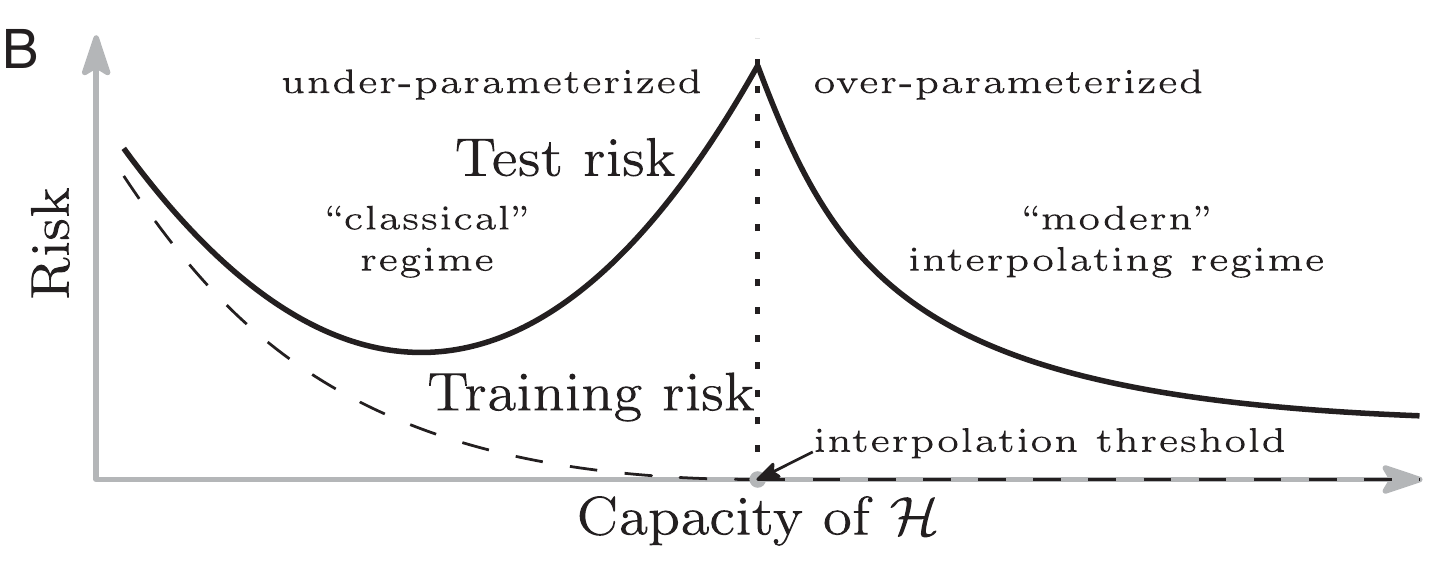
\includegraphics[width=1.2\textwidth]{"Images/Double_Descent.png}
	\par
	\caption{Curve showing the double descent proposition. When the capacity of $\HH$ is large enough the test risk may be lower than that at the local minimum.} \label{fig:Double_Descent}
\end{figure}

\pagebreak

\section{Random Fourier Features} \label{sec:RFFs}
For a feature map $\phi: \RR^d \rightarrow \RR^{d'}$ the kernel trick allows easy computation for positive definite kernel $k$ where $k(x,y) = \inner{\phi(x),\phi(y)}$. We want to find a randomized feature map $z: \RR^d \rightarrow \RR^{\bar{d}}$ such that 
\begin{equation*}
\begin{split}
k(x,y) &= <\phi(x), \phi(y)> \\
&\approx <z^{\Trans}(x), z(y)>.
\end{split}
\end{equation*}
As suggested by \cite{RFF_Rahimi}, for a shift-invariant kernel $k$: $k(x, y) = k(x - y)$), we consider the mapping $z(x) = cos(w^{\Trans}x + b)$, where $w$ is drawn from the probability distribution $p$:
\begin{equation}
p(w) = \frac{1}{2\pi} \int k(h) ~ \text{exp}(-iw^{\Trans}h) ~ \text{d}h
\label{eq:probFourier}
\end{equation} 

when we compute the Fourier transform of the kernel $k$, and $b$ is drawn from the uniform distribution on $[0, 2\pi]$.

We know that the fourier transform of $k(\cdot)$ is a probability distribution from Bochner's theorem:
\begin{thm} \label{thm:Bochner}
	(Bochner \cite{Rudin_1990}).For a continuous kernel $k(x - y)$  it is a positive definite kernel if and only if $k(\cdot)$ is the fourier transform of a non-negative measure.
\end{thm}

We now have:
\[ k(x - y) = \int_{\RR^d} p(w) \text{exp}(iw^{\Trans}(x - y)) ~ \text{d}w = \EE_w[e^{iw^{\Trans}x}(e^{iw^{\Trans}y})^*]. \]
Therefore, we can use $e^{iw^{\Trans}x}(e^{iw^{\Trans}y})^*$ as an (unbiased) estimate of $k(x, y)$.
Let $\phi_w(x) = e^{iw^{\Trans}x}$
We can also use $z_w(x) = \sqrt{2}cos(w^{\Trans}x + b)$ instead of $\phi_w(x)$, as suggested by \cite{RFF_Rahimi}.
\begin{prop}
	For $z_w(x) = \sqrt{2}cos(w^{\Trans}x + b)$, where $w$ is drawn from probability distribution $p$ in \eqref{eq:probFourier} and $b$ drawn from a uniform random variable on $[0, 2\pi]$.
	\[E(z_w(x))z_w(y) = k(x,y)\]
\end{prop}
\begin{proof}
	\begin{equation*}
	\begin{split}
	z_w(x) &= 2 ~ \frac{\sqrt{2}}{2}cos(w^{\Trans}x + b) \\
	&= \frac{1}{\sqrt{2}}~(e^{i(w^{\Trans}x+b)} + e^{-i(w^{\Trans}x+b)}) \\
	&= \frac{1}{\sqrt{2}}~(\phi_w(x)e^{ib} + \phi_w(x)^* e^{-ib})
	\end{split}
	\end{equation*}
	Where $\phi_w(x) = e^{iw^{\Trans}x}$.
	\begin{equation*}
	\begin{split}
	z_w(x)z_y(y) &= \frac{1}{2}[\phi_w(x)\phi_w(y)e^{i2b} + \phi_w(x)^*\phi_w(y)^*e^{-i2b} \\
	&~ + \phi_w(x)\phi_w(y)^* + \phi_w(x)^*\phi_w(y)] \\
	\EE[z_w(x)z_y(y)] &= \frac{1}{2}\EE[\phi_w(x)\phi_w(y)e^{i2b} + \phi_w(x)^*\phi_w(y)^*e^{-i2b}]\\
	&~ + \frac{1}{2}\EE[\phi_w(x)\phi_w(y)^*] + \frac{1}{2}\EE[\phi_w(x)^*\phi_w(y)] \\ 
	\end{split}
	\end{equation*}
	As mentioned earlier in Theorem \ref{thm:Bochner}, $\EE_w[\phi_w(x)\phi_w(y)^*] = k(x - y)$.
	Also $\phi_w(x)\phi_w(y)^* = (\phi_w(x)^*\phi_w(y))^*$.
	\begin{equation*}
	\begin{split}
	\EE[z_w(x)z_y(y)] &= \frac{1}{2}\EE[\phi_w(x)\phi_w(y)e^{i2b} + \phi_w(x)^*\phi_w(y)^*e^{-i2b}]
	+ \frac{1}{2}k(x-y) + \frac{1}{2}[k(x-y)]^* \\
	&= \frac{1}{2}\EE[\phi_w(x)\phi_w(y)e^{i2b} + \phi_w(x)^*\phi_w(y)^*e^{-i2b}] + k(x-y)
	\end{split}
	\end{equation*}
	For real kernel , $k(x - y) = (k(x - y))^*$.
	\begin{equation*}
	\begin{split}
	\EE_{w,b}[\phi_w(x)\phi_w(y)e^{i2b}] &= \frac{1}{2\pi}\int_{\RR^d}\int_{0}^{2\pi} p(w)\phi_w(x)\phi_w(y)e^{i2b} \text{d}b~\text{d}w \\
	&= \frac{1}{2\pi}\int_{\RR^d} p(w)\phi_w(x)\phi_w(y) \int_{0}^{2\pi} e^{i2b} \text{d}b~\text{d}w \\
	&= 0
	\end{split}
	\end{equation*}
	Since $\int_{0}^{2\pi} e^{i2b} \text{d}b = 0$. Similarly, $	\EE_{w,b}[\phi_w(x)^*\phi_w(y)^*e^{-i2b}] = 0$.
	\[ \therefore \EE[z_w(x)z_y(y)] = k(x - y). \]
	
\end{proof}
The variance of the estimate is decreased by using $z$, a $D$ dimensional vector by concatenating $D$ of $z_w$ and normalizing by a constant $\sqrt{D}$. We let:
\[z(x) = \sqrt{\frac{2}{D}} [cos(w_1^{\Trans}x + b_1) ... cos(w_D^{\Trans}x + b_D)] \]
with randomly drawn $w_i$ and $b_i$ as described previously.

\section{Experiment} \label{sec:RFF_Exp}
\subsection{Function Class}
Assume we have datapoints $\{(x_j, y_j)\}_{1 \leq j \leq n}$, where $x_j \in \RR^d$, $y_j \in \RR$.\\
Let $\xi(x;w) := \exp(i w^\Trans x)$.
Consider the class of functions, $\HH_N$ with $N$ number of complex free parameters. That consist of $h_N: \RR \rightarrow \CC$ where:
\[ h_N(x) = \sum_{j=1}^{N} a_j \xi(x;w_j). \]
Where $w_1,..., w_N \in \RR^d$ are sampled independently from the standard Gaussian distribution. With this, $\HH_N$ becomes a better approximation of the RKHS corresponding to the Gaussian RBF kernel when $N$ is huge. We denote the RKHS corresponding ot the Gaussian RBF kernel with $H_\infty$. As per standard machine learning procedure, we want to find $a_1, ..., a_N$ so that the function $h_N \in \HH_N$ is predicts $y$ given unseen $x$ well.
\subsection{Algorithm}
Choose $a = (a_1,..., a_N)$ only through minimization of the square loss, i.e.
\[ \min_{a} \frac{1}{n} \sum_{k=1}^{n}(h_N(x_k) - y_k)^2. \]
However, when the minimizer is not unique (which will be the case when $N > n$), choose $a$ such that it has the smallest L2-norm out of all the minimizers. We give some rationale as to choosing the smallest norm in the section \ref{sec:AppThm}.\\
This choice of norm for $a$ is meant to be similar to the RKS norm $\norm{h}_{\HH_\infty}$. Below, we give a sketch as to the reason:

	Let $f(x)$ be the minimum norm RKHS interpolant function for the datapoints. 
	\begin{equation*}
	\begin{split}
	f(x) &= \sum_{i}\beta_ik(x_i, x)  \because(\text{Representer Theorem}) \\
	&\approx \sum_{i}\beta_iz(x_i)^\text{T}z(x) \\
	&= a^\text{T}z(x) = \hat{f}(x)
	\end{split}
	\end{equation*}
	Where $a = \sum_{i}\beta_iz(x_i) $.
	The norm of the function from the random fourier features approximation is:
	\begin{equation*}
	\begin{split}
	\norm{a} &=   a^\text{T} a = 
	(\sum_{i}\beta_i z^\text{T}(x_i)) (\sum_{i}\beta_i z(x_i)) \\
	&= \sum_i \sum_j \beta_i \beta_j z^\text{T}(x_i)z(x_j)  \\
	&\approx \sum_i \sum_j \beta \beta_j k(x_i, x_j) \\
	&= \norm{f}_{\HH_\infty}
	\end{split}
	\end{equation*}

\subsection{Results}
This was tested on the MNIST dataset, with more information in the original paper.\\
The initial part of the curve as $N < n$ follows a standard U-shaped descent curve, However, after the point of interpolation when there is 0 training risk (when $N = n$), the test loss decreases, even dipping below the previous local minimum as $N$ grows larger (around $N = 2n$). It keeps decreasing as $N$ increases further, moving towards the original kernel solution as seen in Figure \ref{fig:RFF_Exp}.

\begin{figure}
	\centering
	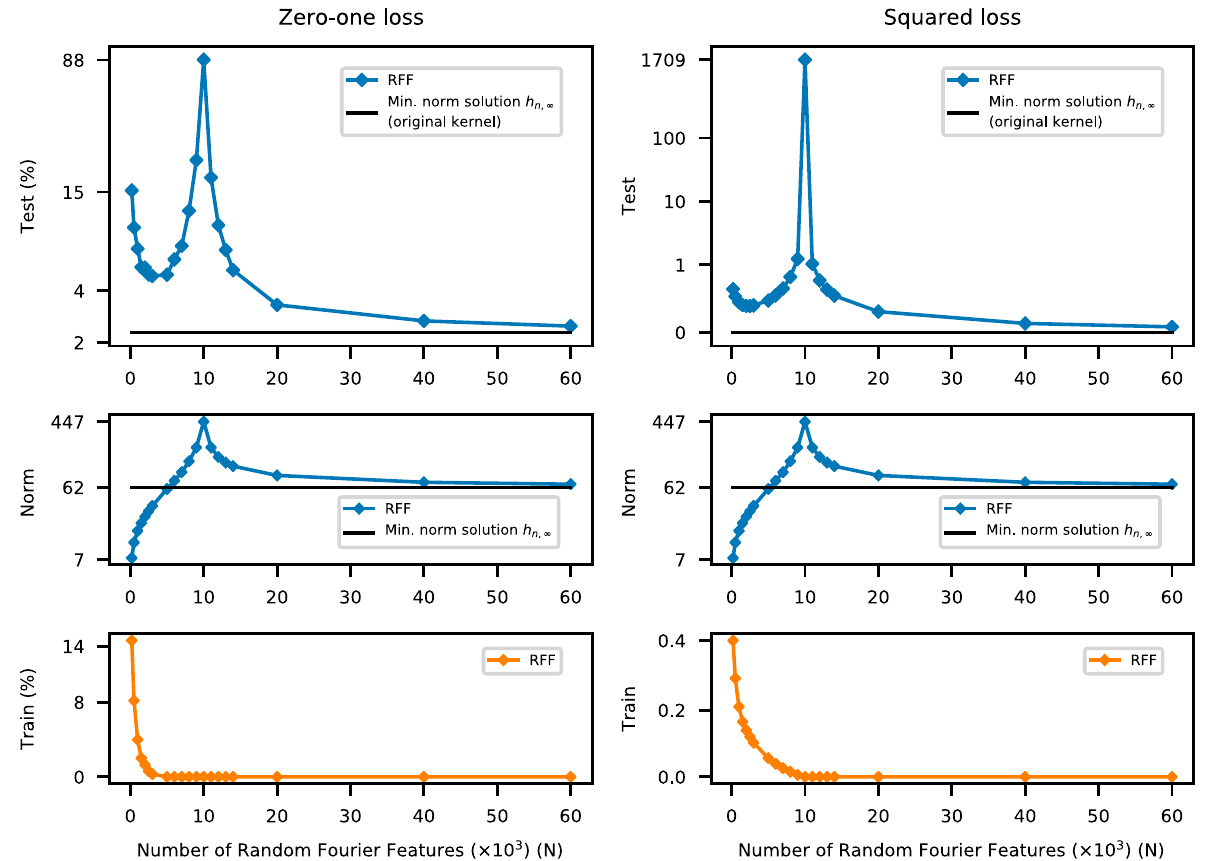
\includegraphics[width=1.3\textwidth]{"Images/RFF_Exp.png}
	\par
	\caption{Experimental Results: RFF function class on MNIST. $n=10^4$, test risk and coefficient norm is in logarithmic scale.} \label{fig:RFF_Exp}
\end{figure}

\section{Plausible Explanations}
Why does the test risk decrease even when increasing $N$ after the point of interpolation?\\
If we look at equation (\ref{eqn:Generalization_Gap}), it seems counter-intuitive to increase the complexity of the function class after the point of interpolation. Afterall the $L_{emp}$ remains at 0, while the complexity of $\HH$ increases, thus increasing the upper bound of the generalization gap. It seems that this upper bound is insufficient in explaining the decrease in test risk.\\
An explanation given by the paper is that the capacity of the function class might not be a good inductive bias (or a good indicator for the inductive bias) for the problem. For example, if the inductive bias is a smooth function, or a smaller norm, or a larger margin (for classification), then by considering a class with a wider range of fucntions, the algorithm may find a function that is able to better fit that inductive bias.\\
For example, in the case of the experiment presented, we are able to find $a$ with smaller L2-norm when we increase $N$, as was shown in the Figure \ref{fig:RFF_Exp}, which might explain the decrease of test risk.

\chapter{Approximation and Estimation}
\section{Notations} \label{sec:Notations}

Let $\pi_m(\RR^d)$ be a multivariate polynomial with $d$ variables and degree $\leq m$, i.e. 
\[ \pi_m(\RR^d) = \{ p(x) = \sum_{k \leq m} c_k x^k \} \] 	
\\
Let $C^k(X)$ be the set of functions on $X$ that are $k$ times continuously differentiable. \\
For a point $x \in \RR^d$, it has the components of its coordinates $\chi_1, .., \chi_d$, whereas we represent $n$ points in $\RR^d$ as $x_1, .., x_n$.\\
We denote $\NN_0$ as the set of non-negative integers.
We denote the multi-index vector with its components as $\alpha = (\alpha_1, ..., \alpha_d)^\Trans \in \NN_{0}^{d}$, and $|\alpha| := \norm{\alpha}_1$ For $X \subseteq \RR^d$, $f \in C^k(X)$, $|\alpha| \leq k$ and $x \in \RR^d$, we denote:
\[ D^\alpha f := \frac{\partial^{|\alpha|}}{\partial\chi_1^{\alpha_1} \cdot\cdot\cdot \partial\chi_d^{\alpha_d}} f \]

\begin{defn}
	Consider the set of points $X = {x_1, ..., x_n} \subseteq \RR$ and $\pi_m(\RR^d)$ with $n \geq \dim(\pi_m(\RR^d)$. $X$ is called $\pi_m(\RR^d)$-unisolvent if there is no polynomial in $\pi_m(\RR^d)$ (besides the zero polynomial) that is zero on all the points.
\end{defn}


\section{Interpolation Estimates}

Let $X = {x_1, ..., x_n} \subseteq \RR$  be a set of points that is $\PPP$ unisolvent. For $p_1, .., p_Q$ that form a basis of $\PPP$, let $P = (p_j(x_i)) \in \RR^{n\times Q}$. Let $\Phi$ be a positive definite kernel and $A = (\Phi(x_i, x_j)) \in \RR^{n\times n}$. We let $e^{(j)}$ represent the $j$th unit vector.
Consider the linear system:
\begin{equation} \label{eqn:InterpolateMat}
\begin{pmatrix}
A & P \\
P^\Trans & 0 \\
\end{pmatrix}
\begin{pmatrix}
\alpha^{(j)} \\ \beta^{(j)}
\end{pmatrix}
=
\begin{pmatrix}
e^{(j)} \\ 0
\end{pmatrix}.
\end{equation}
This linear system is uniquely solvable for $j \in \{1, 2, .., n\}$.

\begin{proof}
	For $\begin{pmatrix}
	\alpha \\ \beta
	\end{pmatrix}$ that lies in the null space of the matrix
	$\begin{pmatrix}
	A & P \\
	P^\Trans & 0 \\
	\end{pmatrix}$, we have the 2 equations:
	\begin{equation*}
	\begin{split}
	A \alpha + P \beta &= 0,\\
	P^\Trans \alpha = 0. \\
	\end{split}
	\end{equation*}
	From the first equation, multiplying both sides by $\alpha^\Trans$, we get:
	\begin{equation*}
	\begin{split}
	\alpha^{\Trans} A \alpha + \alpha^{\Trans} P \beta &= 0\\
	\implies \alpha^{\Trans} A \alpha + (P^\Trans \alpha)^\Trans \beta &= 0\\
	\implies \alpha^{\Trans} A \alpha &= 0\\
	\end{split}
	\end{equation*}
	Since we know $\Phi$ is a positive definite kernel, then $\alpha = 0$, so we know $P \beta = 0$. Since $X$ is $\PPP$-unisolvent, so $\beta = 0$. Hence, the linear system (\ref{eqn:InterpolateMat}) is uniquely solvable.
\end{proof}
Let $u_j^*, V_X$ be defined such that:
\begin{equation}
\begin{split}
u_j^* &:= \sum_{i=1}^{n} \alpha_i^{(j)} \Phi(\cdot, x_i) + \sum_{k=1}^{Q} \beta_k^{j} p_k \label{eq:ustar}\\
V_X &:= \{ \sum_{i=1}^{n} \alpha_i \Phi(\cdot, x_i) ~ : \sum_{i=1}^{n} \alpha_i p(x_i) = 0, p \in \PPP  \} + \PPP.
\end{split}
\end{equation}
So we have $u_j^* \in V_X$ and \[ u_i^*(x_j) =  \begin{cases} 
1 & i=j \\
0 & i \neq j.\\
\end{cases}
\]

Also, for all $f \in V_X$, we have 
\begin{equation} \label{eqn:finVx}
f = \sum_{i=1}^{n} u_i^* f(x_i).
\end{equation}
For our next theorem, we further define:
\begin{equation}
\begin{split}
R(\cdot) &:= (\Phi(\cdot, x_1),..., \Phi(\cdot, x_n))^\Trans \in \RR^n\\
S(\cdot) &:= (p_1(\cdot),..., p_Q(\cdot))^{\Trans} \in \RR^Q \\
\end{split}
\end{equation}
\begin{thm}
	For $\Phi$ a positive definite kernel on $\Omega \subseteq \RR^d$ and points $X = \{ x_1,..., x_n \} \subseteq \Omega$ is $\PPP$-unisolvent. There exists functions $v_i^*(\cdot)$ for $i = \{ 1, 2, .., Q \} $ such that for $u^*(x) = (u^*_1(x), ..., u^*_n(x)$ where $u^*_i$ is defined in (\ref{eq:ustar}). we have:
	\begin{equation} \label{eqn:vstar}
	\begin{pmatrix}
	A & P \\
	P^\Trans & 0 \\
	\end{pmatrix}
	\begin{pmatrix}
	u^*(x)\\ v^*(x)
	\end{pmatrix}
	=
	\begin{pmatrix}
	R(x)\\ S(x)
	\end{pmatrix}
	\end{equation}
\end{thm}
\begin{proof}
	One of the things to be proven is that $P^\Trans u^*(x) = S(x)$. Since $\PPP \subseteq V_X$, then $(p_1,..., p_Q) \in V_X$, so by (\ref{eqn:finVx}), we have: $p_i(x) = \sum p_i(x_j)u_i^*(x)$, showing $P^\Trans u^*(x) = S(x)$.\\
	Next, we need to show that there exists $v*$ such that $Au^*(x) + Pv^*(x) = R(x)$, so we need to show $Au^*(x) - R(x) \in P(\RR^Q)$.\\
	$(P(\RR^Q))^\perp$ is the null space of its transpose. Consider $\omega \in \text{null}(P^\Trans) \subseteq \RR^n$, so we need to show that $\omega^\Trans (Au^*(x) - R(x)) = 0$, i.e. $\omega^\Trans Au^*(x) = \omega^\Trans R(x)$.\\
	\begin{equation*}
	\begin{split}
	P^\Trans \omega &= 0\\
	\implies \omega^\Trans R(x) &\in V_X\\
	\omega^\Trans R(\cdot) &= \sum_{i=1}^{n}u_i(\cdot)\omega^\Trans R(x_i) ~~(\because (\ref{eqn:finVx}))\\
	&= \sum_{i=1}^{n} \sum_{j=1}^{n} u_i^*(\cdot) \omega_j \Phi(x_i, x_j) \\
	&= \gamma^\Trans A u^*(\cdot).\\
	\end{split}
	\end{equation*}
\end{proof}

\begin{lem}
	$v^*$ has the property where, for $v_i$ with $1 \leq i \leq Q$, we have: $v_i(x_j) = 0$ for $1 \leq j \leq n$.
\end{lem}
\begin{proof}
	\begin{equation*}
	\begin{split}
	A u^*(x_i) &= A e^{(i)} \\
	&= \begin{pmatrix}
	\Phi(x_i, x_1) \\  \vdots \\ \Phi(x_i, x_n)\\
	\end{pmatrix} \\
	A u^*(x_i) + P v^*(x_i) &= R(x_i) = A u^*(x_i) \\
	\implies P v^*(x_i) = 0 \\
	\end{split}
	\end{equation*}
	Since $X$ is $\PPP$-unisolvent, $v^*(x_i) = 0$.
\end{proof}
Also, from Theorem 11.1 of \cite{ScatteredDataApproximation}, we are able to rewrite an interpolant as:
\begin{equation} \label{eqn:InterDecomp}
s_{f,X}(\cdot) = \sum_{i=1}^{n} f(x_i)u_i^*(\cdot).
\end{equation}

By differentiating \ref{eqn:vstar}, we have:
\begin{equation}
\begin{pmatrix}
A & P \\
P^\Trans & 0 \\
\end{pmatrix}
\begin{pmatrix}
D^a u^*(x)\\ D^a v^*(x)
\end{pmatrix}
=
\begin{pmatrix}
D^a R(x)\\ D^a S(x)
\end{pmatrix}.
\end{equation}

We will define the power function, as defined in Definition 11.2 in \cite{ScatteredDataApproximation}:
\begin{defn}
	Suppose $X \in \RR^d$ is open, with $k: X \times X \rightarrow \RR$ be a positive definite kernel. For $\alpha \in \NN_0^d$, $\hat{X} = {x_1, x_2, ..., x_n} \subseteq X$ the power function $P^{(\alpha)}_{k,\hat{X}}(x)$ is defined by:
	\begin{equation*}
	\begin{split}
	(P^{(\alpha)}_{k,\hat{X}}(x))^2 &:= D_1^\alpha D_2^\alpha k(x, x) 
	- 2 \sum_{j=1}^n D^{\alpha}u_j^*(x)D_1^\alpha k(x, x_j) \\
	&+ \sum_{i,j = 1}^{n} D^\alpha u_i^*(x) D^\alpha u_j^*(x) k(x_i, x_j).
	\end{split}
	\end{equation*}
\end{defn}
In Theorem 11.4 of \cite{ScatteredDataApproximation}, we have:
\begin{thm}\label{thm:PowerBound}
	For an open set $\Omega \subseteq \RR$ and a positive definite kernel $k \subseteq C^{2k}(\Omega \times \Omega)$, and the set of points $X = \{x_1,..., x_n\} \subseteq \Omega$ is $\PPP$-unisolvent. Let $\HH$ be RKHS corresponding to the kernel $k$, a function $f \in \HH$ and its interpolant be $s_{f,X}$. For every $x \in \Omega, a \in \NN_0^d, |a| \leq k$, we have:
	\begin{equation}
	|D^af(\cdot) - D^as_{f,X}(\cdot)| \leq P^{a}_{k,X}(\cdot) \norm{f}_{\HH}.
	\end{equation}
\end{thm}
\begin{proof}
	We shall proof the case of $a = 0$, which is the case which will be used in a later theorem.
	First, we note that:
	\begin{equation*}
	\begin{split}
	\norm{k(\cdot,x) - \sum_{i=1}^{n}u_ik(\cdot, x_i)}^2_\HH &= k(x,x) - 2\sum_{i=1}^{n}u^*_ik(x,x_i) + \sum_{i,j=1}^{n}u^*_iu^*_jk(x_i,x_j) \\
	= (P^{(0)}_{k,X}(x))^2.
	\end{split}
	\end{equation*}
	Next, using (\ref{eqn:InterDecomp}), we have:
	\begin{equation*}
	\begin{split}
	s_{f,X}(x) &= \sum_{i=1}^{n} f(x_i) u_i^*(x) \\
	&= \sum_{i=1}^{n} u_i^*(x) \inner{f, k(\cdot, x_i)}_\HH ~~ (\because \text{reproduction property}) \\
	&= \inner{f, \sum_{i=1}^{n}u_i^*(x) k(\cdot, x_i)} \\
	\implies |f(x) - s_{f,X}(x)| &= | \inner{f, k(\cdot, x)}_\HH -  \inner{f, \sum_{i=1}^{n}u_i^*(x) k(\cdot, x_i)} | \\
	&= |\inner{f,  k(\cdot, x) - \sum_{i=1}^{n}u_i^*(x) k(\cdot, x_i)}_\HH| \\
	&\leq \norm{f}_\HH \norm{k(\cdot, x) - \sum_{i=1}^{n}u_i^*(x) k(\cdot, x_i)}_\HH ~~ (\because \text{Cauchy-Schwarz inequality}) \\
	&= \norm{f}_\HH P^{(0)}_{k,X}(x).
	\end{split}
	\end{equation*}
\end{proof}
\begin{defn}
	The fill distance (or sometimes referred to as 'fill' for short) for a set of points $X = \{x_1, ..., x_N\} \subseteq \Omega$ for a bounded domain $\Omega$ is defined to be
	\[
	h_{X,\Omega} \coloneqq \sup_{x \in \Omega}\min_{1 \leq j \leq N} \norm{x- x_j}_2.
	\]
\end{defn}

Theorem 11.22 in \cite{ScatteredDataApproximation}:
\begin{thm} \label{thm:interpolate}
	Let $\Omega$ be a cube in $\RR^d$ and $k = \phi(\norm{\cdot}_2)$ be a positive definite function with $f = \phi(\cdot)$ satisfying the condition that there exists, $l_0$ and constant $M > 0$ such that for all $r > 0$ and $l > l_0$, $|f^{(l)}(r)| \leq l!M^l$. Then there exists a constant $c > 0$ such that the error between a function $f \in \RKHSGauss$ and its interpolant $s_{f,X}$ for all data points $X = \{x_1, ..., x_n\}$ can be bounded by:
	\begin{equation*}
	\norm{f - s_{f,X}}_{L_\infty(\Omega)} \leq \text{exp}(-c/h_{X,\Omega})|f|_{\RKHSGauss}
	\end{equation*}
	with sufficiently small fill $h_{X,\Omega}$.
\end{thm}
\begin{proof}
	From Theorem 11.9 in \cite{ScatteredDataApproximation}, we have:
	\[ P_{\Phi, X}^2(x) \leq [1 + c_1(2N)]^2 \norm{f - p}_{L_\infty(G)} \]
	Where $G$ is on the interval $[0, 4(c_2(2N))^2h^2]$, $x \in \Omega$, $p \in \pi_n(\RR)$, $h = h_{X, \Omega}$.
	
	From Theorem 11.21 in \cite{ScatteredDataApproximation},: we have for sufficiently small fill distance $\fillDist \leq \frac{c_0}{2n}$, there exists a constant $\gamma_d$, where the constants $c_1, c_2$ can be replaced by:
	\begin{equation*}
	\begin{split}
	c_1(2n) &= \exp(2d\gamma_d(2n+1))\\
	c_2(2n) &= 2c_2n
	\end{split}
	\end{equation*}
	So $G$ is on the interval $[0, 16N^2c_2^2h^2]$
	For $p$ the Taylor series of $f$ about 0, and up to the term $t^N$, we then have:
	\begin{equation*}
	\begin{split}
	|f(t) - p(t)| &\leq t^{N+1}\frac{|f^{n+1}(t')|}{(n+1)!} \\
	&\leq M^{N+1}t^{N+1} ~ \text{ (By assumption)} \\
	\implies {\norm{f - p}}_{L_\infty(G)} &\leq (M \cdot 16N^2c_2^2h^2)^{N+1} \\
	&= (C_0 N^2 h^2)^{N+1} ~ \text{ for constant }C_0 = Mc_2^2 \\
	\end{split}
	\end{equation*}
	Also, we have:
	\begin{equation*}
	\begin{split}
	[1 + c_1(2N)]^2 &= [1 + \exp(2d\gamma_d(2N + 1))]^2 \\
	&\leq [2\exp(2d\gamma_d(2N + 1))]^2 \\
	&= 4\exp(4d\gamma_d(2N + 1)) \\
	&= \exp(\log 4 + 4d\gamma_d(2N + 1)) \\
	&\leq \exp(C_1(N+1)) ~ \text{ for sufficiently large }C_1.\\
	\end{split}
	\end{equation*}
	We then have:
	\begin{equation} \label{eqn:P2bound}
	\begin{split}
	P^2_{\Phi, X}(x) &\leq [1 + c_1(2N)]^2 \norm{f - p}_{L_\infty(G)} \\
	&\leq \exp(C_1(N+1))( C_0 N^2 h^2)^{N+1} \\
	&= (C_0 N^2 h^2\exp(C_1))^{N+1} \\
	&= (C_2 N^2 h^2)^{N+1} ~ \text{ for constant }C_2 = C_0\exp(C_1). \\
	\end{split}
	\end{equation}
	For $C_3 = \min(\frac{c_0}{2}, \frac{1}{\sqrt{e C_2}})$, and $N$ such that
	\[ \frac{C_3}{N+1} \leq h \leq \frac{C_3}{N} \], which gives us:
	\begin{equation*}
	\begin{split}
	h &\leq \frac{c_0}{2N}, \\
	-(N+1) &\leq -C_3/h, \\
	N^2h^2 \leq &C_3^2 \leq \frac{1}{eC_2} \\
	\implies C_2N^2h^2 &\leq  1/e. \\
	\end{split}
	\end{equation*}
	We then have:
	\begin{equation*}
	P^2_{\Phi, X}(x) \leq e^{-(N+1)} \leq e^{-C_3/h}. 
	\end{equation*}
	Now, using $C= C_3/2$ and $|f(x) - s_{f, X}(x)| \leq P_{\Phi, X}(x) |f|_{\RKHSGauss}$ (from Theorem (\ref{thm:PowerBound})), we have:
	\[ |f(x) - s_{f, X}(x)| \leq e^{-C/\fillDist} |f|_{\RKHSGauss}, \]
	which is what we wanted to prove.
\end{proof}

\begin{thm}
	With the same conditions as Theorem \ref{thm:interpolate}, except that $f$ satisfies the stricter condition $|f^{(l)}(r)| \leq M^l$, we can get a better error bound of:
	\[ \norm{f - s_{f,X}}_{L_\infty(\Omega)} \leq \exp(\frac{c \log(\fillDist)}{\fillDist})\norm{f}_{\RKHSGauss}. \]
\end{thm}
\begin{proof}
	The inequality at \ref{eqn:P2bound} becomes:
	\[ P^2_{\Phi, X}(x) \leq  \frac{(C_2 N^2 h^2)^{N+1}}{(N+1)!}. \]
	
	Using Stirling's inequality $1/n! \leq (e/n)^n$, we have:
	\[ P^2_{\Phi, X}(x) \leq (eC_2 N h^2)^{N+1}. \]
	Similarly, with $C_3 = \min(\frac{c_0}{2}, \frac{1}{e C_2})$, and $N$ such that
	\[ \frac{C_3}{N+1} \leq h \leq \frac{C_3}{N}, \] we then get \[ eC_2Nh \leq 1, \] which gives us:
	\[ P^2_{\Phi,X}(x) \leq h^{N+1} \leq h^{C_3/h} = e^{C_3 \log h / h}. \]
	Following the steps of the previous theorem then gives us our result.
\end{proof}
\section{Approximation Theorem} \label{sec:AppThm}
\subsection{Fill Distance of points in a Cube}
First, we need the result that: with $h_{X,\Omega}$ as the fill on the order of $O(n/\log n)^{-1/d}$ (using the theorem S1 in Belkin's paper). We give a proof sketch for this:

Whern $n$ is big enough, we (approximately) divide the cube $\Omega$ into $n$ smaller subcubes, where each subcube has $1/n$ the volume of $\Omega$ (Let the volume of $\Omega$ be 1 for simplicity).\\
Let $g_k$ be a vertice of one of the subcubes. Let $N$ be the number of vertices of the subcubes.
Let's say all $x_i$ are not within $r$ distance from a point $g$.\\ Then $\min_{1 \leq i \leq n} \norm{g - x_i} > r > 0 $ i.e. 
$x_i \notin B(g, r), 1\leq i\leq n$.
\begin{equation*}
\begin{split}
\PP(x_i \notin B(g, r), 1\leq i\leq n) &= \prod_{i=1}^{n} \PP(x_i \notin B(g, r)) \\
&= [\PP(x_i \notin B(g, r))]^n \\
&= [1 - \PP(x_i \in B(g, r))] \\
&= (1 - c_d r^d)^n \\
&\approx \exp(-c_d r^d n). 
\end{split}
\end{equation*}
Where $c_d$ is some constant. It arises due to ratio of volume of ball vs volume of where $x_i$ can be.
The distance from a point $x$ in the cube to some $x_i$ $\leq$ dist($x, g_k$) + dist($g_k, x_i$).\\
For $g_k$ being one of the vertices of the subcube $x$ resides in. For the subcube with length $a$ and dimension $d$ and volume $n^{-1}$, since 
\[ a_d = n^{-1} \implies a = n^{-1/d}. \]
So the end-to-end distance in the subcube is $a\sqrt{d} = n^{-1/d}\sqrt{d}$, which goes to 0 for big $n$, so dist($x, g_k$) will be small.\\
The distance from a point $x$ in the cube to some $x_i$ $\approx$ dist($g_k, x_i$) for large $n$.
\begin{equation*}
\begin{split}
\PP(h_{X,\Omega} > r) &\approx \PP(\exists \text{ vertice } g_k | x_i \notin B(g_k, r), 1\leq i\leq n)\\
&= \PP(\bigcup_{k} \{ x_i \notin B(g_k, r), 1 \leq i \leq n\} ) \\
&\leq \sum_{k=1}^{N}\PP(x_i \notin B(g_k, r), 1 \leq i \leq n) \\
&= \sum_{k=1}^{N} \exp(-c_d r^d n)\\
&\leq 2^d n \exp(-c_d r^d n)\\
&= \exp(d\log 2+\log n - c_d r^d n )
\end{split}
\end{equation*}
$\PP(h_{X,\Omega} > r) \rightarrow 0$ when:
\begin{equation*}
\begin{split}
c_dr^dn &>> \log n\\
\implies ~~ r &>> (\frac{\log n}{n})^{1/d} c_d^{1/d}.
\end{split}
\end{equation*}
i.e. We have a low probability that $\PP(h_{X,\Omega} > r)$ if r grows with respect to $(\frac{n}{\log n})^{-1/d}$ (for large $n$).  



The below theorem gives us some justification as to why the minimum norm interpolating function was chosen, though this only works under noiseless conditions:
% Might need to rephrase this part to avoid plag
\begin{thm} \label{thm:approx}
	Fix $h^* \in \RKHSGauss $  .
	Let $(x_1,y_1), ..., (x_n,y_n)$ be i.i.d. random variables where $x_i$ drawn uniformly at random from a compact cube $\Omega \subseteq \mathbb{R}^d $,
	$y_i = h^*(x_i) \: \forall i$. There exists $A, B > 0$ such that for any interpolating $h \in \mathcal{H}_\infty $ with high probability
	\begin{equation*}
	\sup_{x \in \Omega} \abs{h(x) - h^*(x)} A e^{-B(n/ \log n)^{1/d}} (\norm{ h^*}_{\mathcal{H}_\infty} + \norm{h}_{\mathcal{H}_\infty})
	\end{equation*}
\end{thm}

\begin{proof}
	We consider $f(x) := h(x) - h^*(x)$. Since $h$ is interpolating, we have $f(x_i) = 0$ for all $x_i$. The interpolant of $f$, $s_{f,X}$ will then be the zero function. Thus, we have:
	\begin{equation*}
	\begin{split}
	\norm{f}_{L_\infty(\Omega)} &= \sup_{x \in \Omega} \vert h(x) - h^*(x)\vert \\
	&< \exp(-c(n/\log n)^{1/d})\norm{f}_{\RKHSGauss} \\
	&\leq \exp(-c(n/\log n)^{1/d}) (\norm{h^*}_{\RKHSGauss} + \norm{h}_{\RKHSGauss})
	\end{split}
	\end{equation*}
\end{proof}
Another form we can have is using Proposition 14.1 in \cite{ScatteredDataApproximation}:
\begin{prop}
	Let $\Omega \subseteq \RR^d$ be bounded and measurable. Suppose $X = \{x_1, ... , x_N\} \subseteq \Omega$ is quasi-uniform with respect to  $c_{qu} > 0$. Then there exists constants $c_1, c_2 > 0$ depending only on space dimension $d$, on $\Omega$ and on $c_{qu}$ such that:
	\[c_1N^{-1/d} \leq h_{X,\Omega} \leq c_2N^{-1/d}. \]
\end{prop}
With the definition of quasi-uniformness being:
\begin{defn}
	For the separation distance of $X = \{x_1, ... , x_N\}$ being defined as $q_x \coloneqq \half \min_{i\neq j} \norm{x_i - x_j}_2$.
\end{defn}
We can then use the above proposition with $n$ replacing $n/\log n$ in Theorem \ref{thm:approx} for a better bound of:
\[ \sup_{x \in \Omega} \abs{h(x) - h^*(x)} < A e^{-B(n)^{1/d}} (\norm{h^*}_{\mathcal{H}_\infty} + \norm{h}_{\mathcal{H}_\infty}) \]
if the quasi-uniformness conditions are fulfilled.
In either case, by choosing a the smallest norm for $h$, we can see that it corresponds to the smallest upperbound for $\vert h(x) - h^*(x)\vert$. \\
In the next subsection, we have another rationale for choosing a smaller $\norm{h}_{\RKHSGauss}$:
\subsection{Regularity of Functions}
Let the $\RR$-RKHS $\HH$ consist of functions over $X$. The functions fulfill a Lipschitz-like condition with the Lipschitz constant being the RKHS norm of the function $\norm{f}_{\RKHSGauss}$.\\
For the positive definite symmetric kernel $k$ corresponding to $\HH$, we have for all $x, x' \in X$:
\begin{equation*}
\begin{split}
|f(x) - f(x')| &= |\inner{f, k(\cdot, x)}_{\RKHSGauss} - \inner{f, k(\cdot, x')}_{\RKHSGauss}| \\
&= |\inner{f, \Phi(x) - \Phi(x')}_{\RKHSGauss}| ~ \text{ where }  \Phi(x)(\cdot) = k(\cdot, x)\\
&\leq \norm{f}_{\RKHSGauss} d(x, x'),
\end{split}
\end{equation*}
where $d(x, x')$ is the pseudometric defined by:
\[ d^2(x, x') = k(x, x) - 2k(x, x') + k(x', x'). \]
Intuitively, we can see the "speed" of which the function can change is bounded by the norm of the function in the RKHS space.

\chapter{Other Notes}
\section{Weaknesses}
Huge sample size, density of adversarial examples.

% If you want to include appendices, just use the \appendix command and then make chapters as normal
\appendix
\chapter{Your first appendix}

See \url{https://www.overleaf.com/read/qyhckhfyfvmb} on Overleaf for useful examples of formatted text, typing in IPA, etc.

% For the bibliography style, I load `sp.bst', the style used by the LSA in the journal `Semantics and Pragmatics'. For how to include in-line citations with page numbers and other conventions, refer to nus-el-ht.sty. 
\backmatter
\bibliography{el-ht.bib}
\bibliographystyle{sp}
\end{document}

